% 本原稿用の条件マクロ
%章ごとにコンパイルできるようにするための設定.
%このマクロが定義されていない場合,チャプター内は個別のTEXソースとして扱われる.
\expandafter\ifx\csname MasterFile\endcsname\relax
\documentclass[a4j,twoside,12pt,dvipdfmx]{thesis} % 修論・卒論など (ページが右端にでる) 
\usepackage{amsmath, amssymb}
\usepackage{mysettings}
\usepackage{graphicx}
\usepackage{color}
\usepackage{comment}

\begin{document}

\addtocounter{chapter}{+1}

\setlength{\baselineskip}{1.95zw}
\setlength{\textheight}{30\baselineskip}
\mainmatter

\fi
% これより上は削除しちゃダメ
% 本原稿用の条件マクロここまで
%
%\newcommand{\argmax}{\mathop{\rm arg~max}\limits}
\newcommand{\argminnnn}{\mathop{\rm arg~min}\limits}
\renewcommand\thefootnote{\arabic{footnote})}
\def\vector#1{\mbox{\boldmath $#1$}}

\chapter{関連研究}\label{rel}
% ここに本文
本章では,本研究で取り扱っている基礎知識について説明する.本章の構成は次の通りである.\ref{rel:preKnowledge}節では事前知識について述べる. \ref{rel:GNN}節ではグラフニューラルネットワークについて述べる.

\section{事前知識}\label{rel:preKnowledge}
本節では, 研究を行うにあたって必要な事前知識について述べる.
\subsection{トランスダクティブ学習, 帰納学習}
本項ではトランスダクティブ (Transductive) 学習, 帰納 (Inductive) 学習の 2 つの学習について説明をする.
トランスダクティブ学習とは, 学習時にデータは存在するもののラベルが割り振られていないデータに対して, 推論を行う学習である. その様子を図 \ref{fig:Transductive} に示す.

\begin{figure}
  \centering
  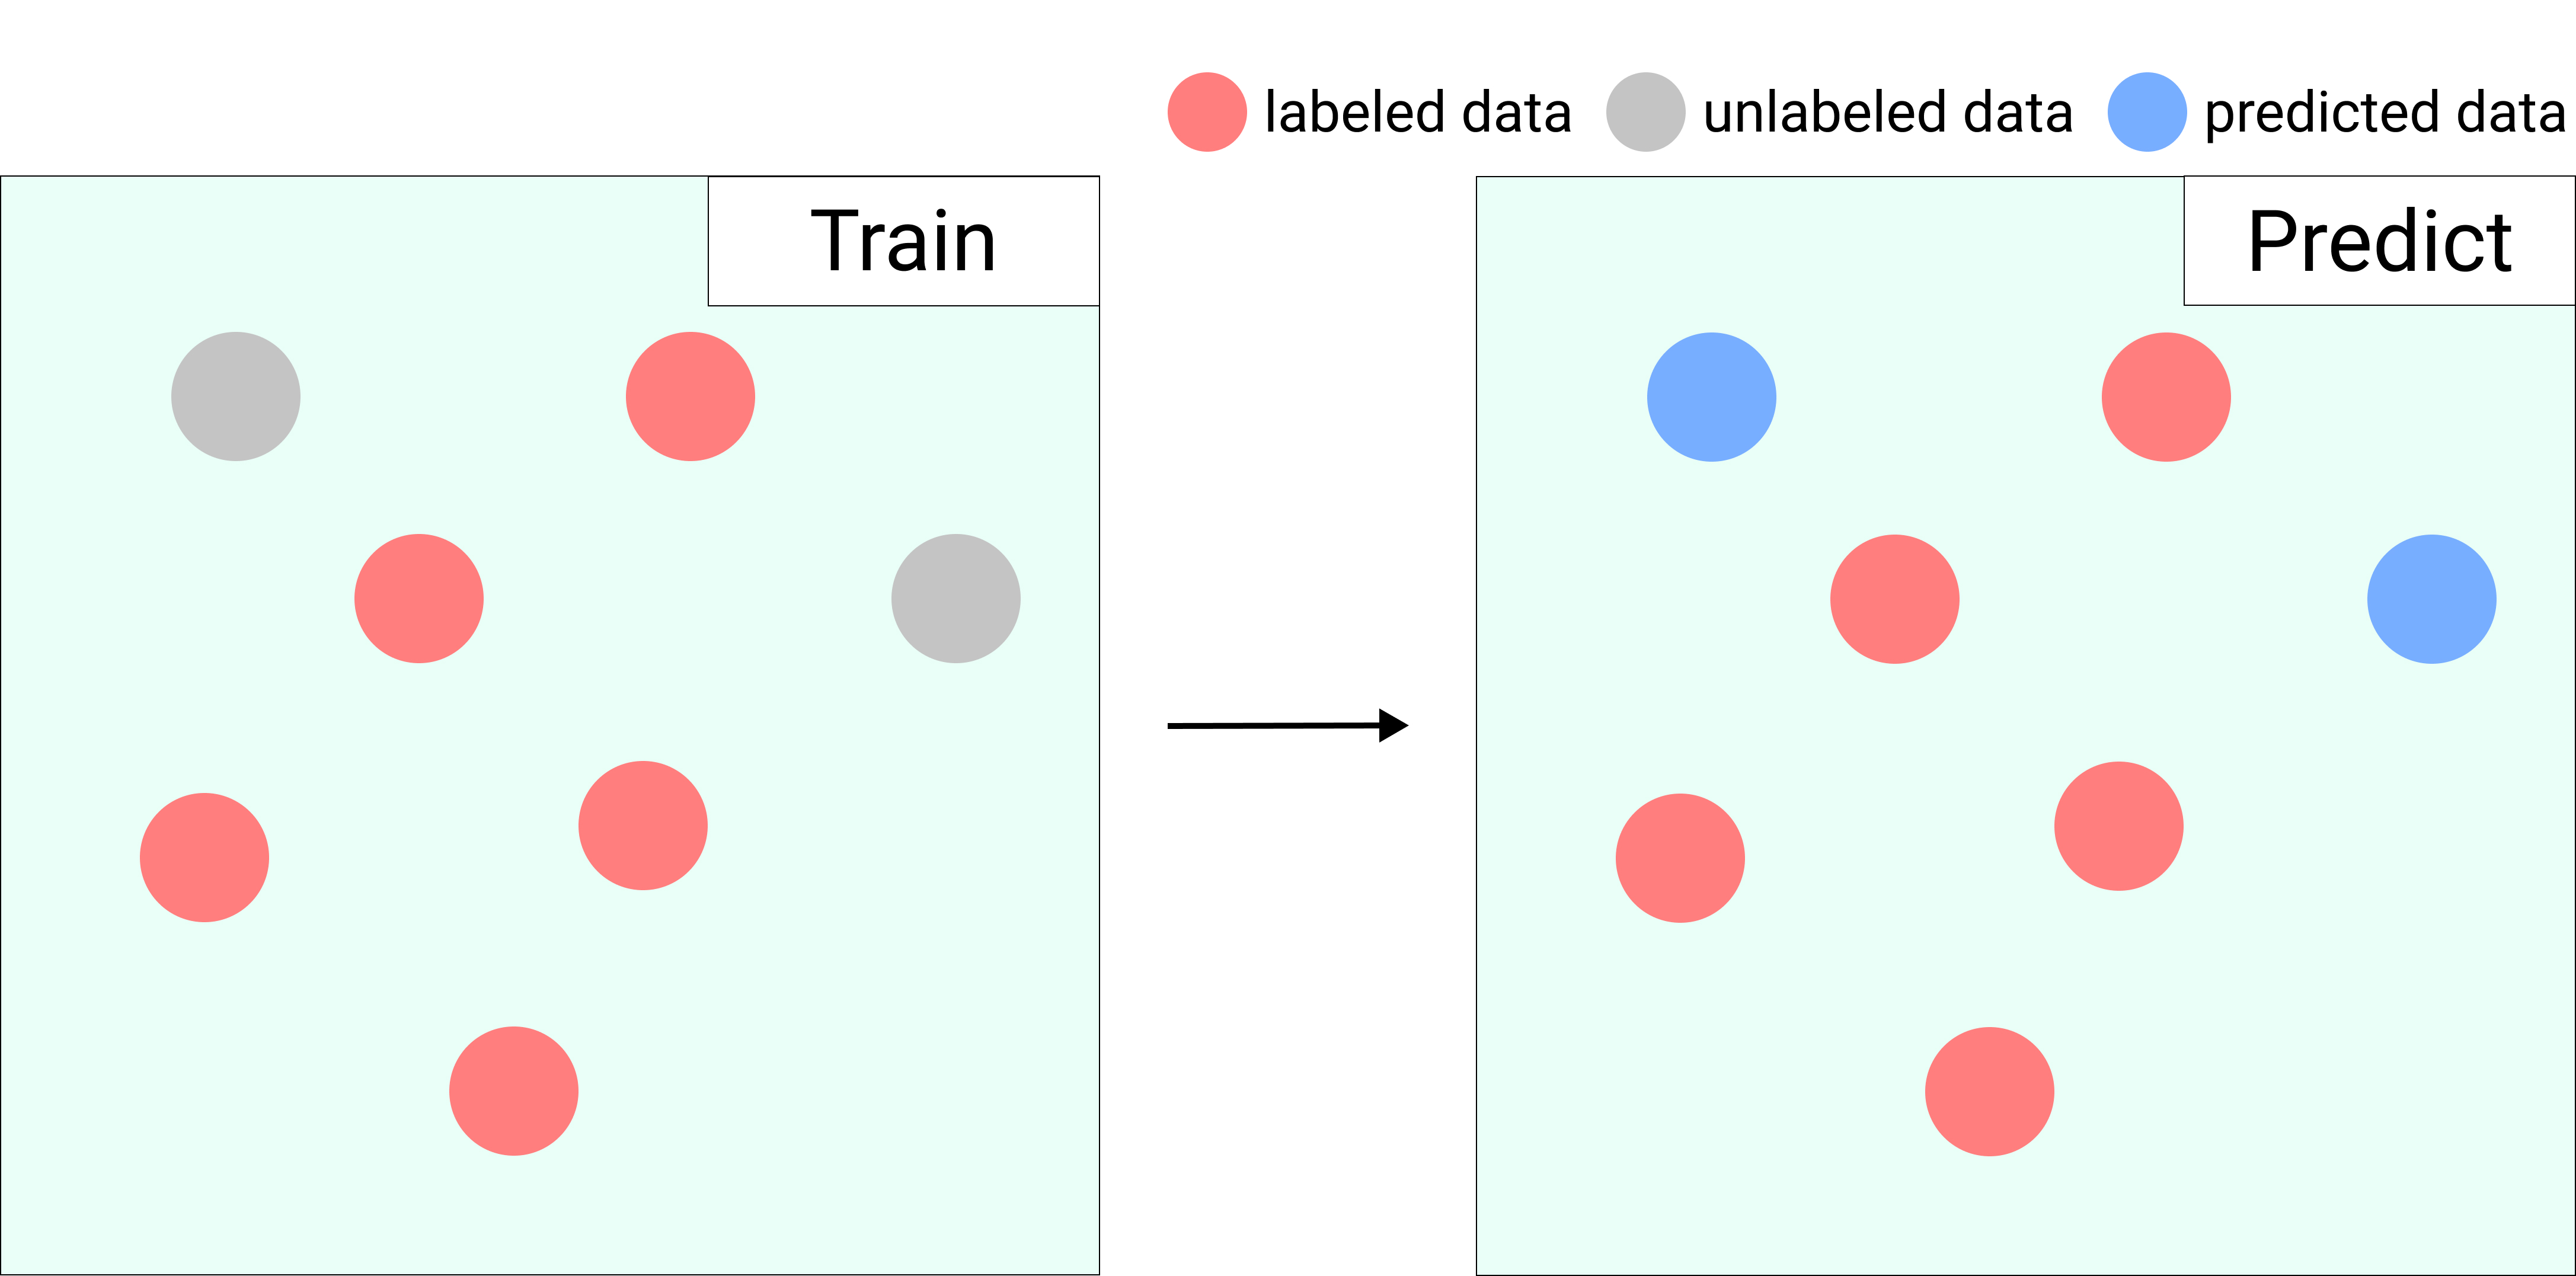
\includegraphics[width=\linewidth]
  {img/Transductive.jpg}
  \caption{トランスダクティブ学習}
  \label{fig:Transductive}
\end{figure}

それに比べて帰納学習とは, 学習時に存在しなかったデータに対しての推論を行う学習である. その様子を図 \ref{fig:Inductive} に示す.


\begin{figure}
  \centering
  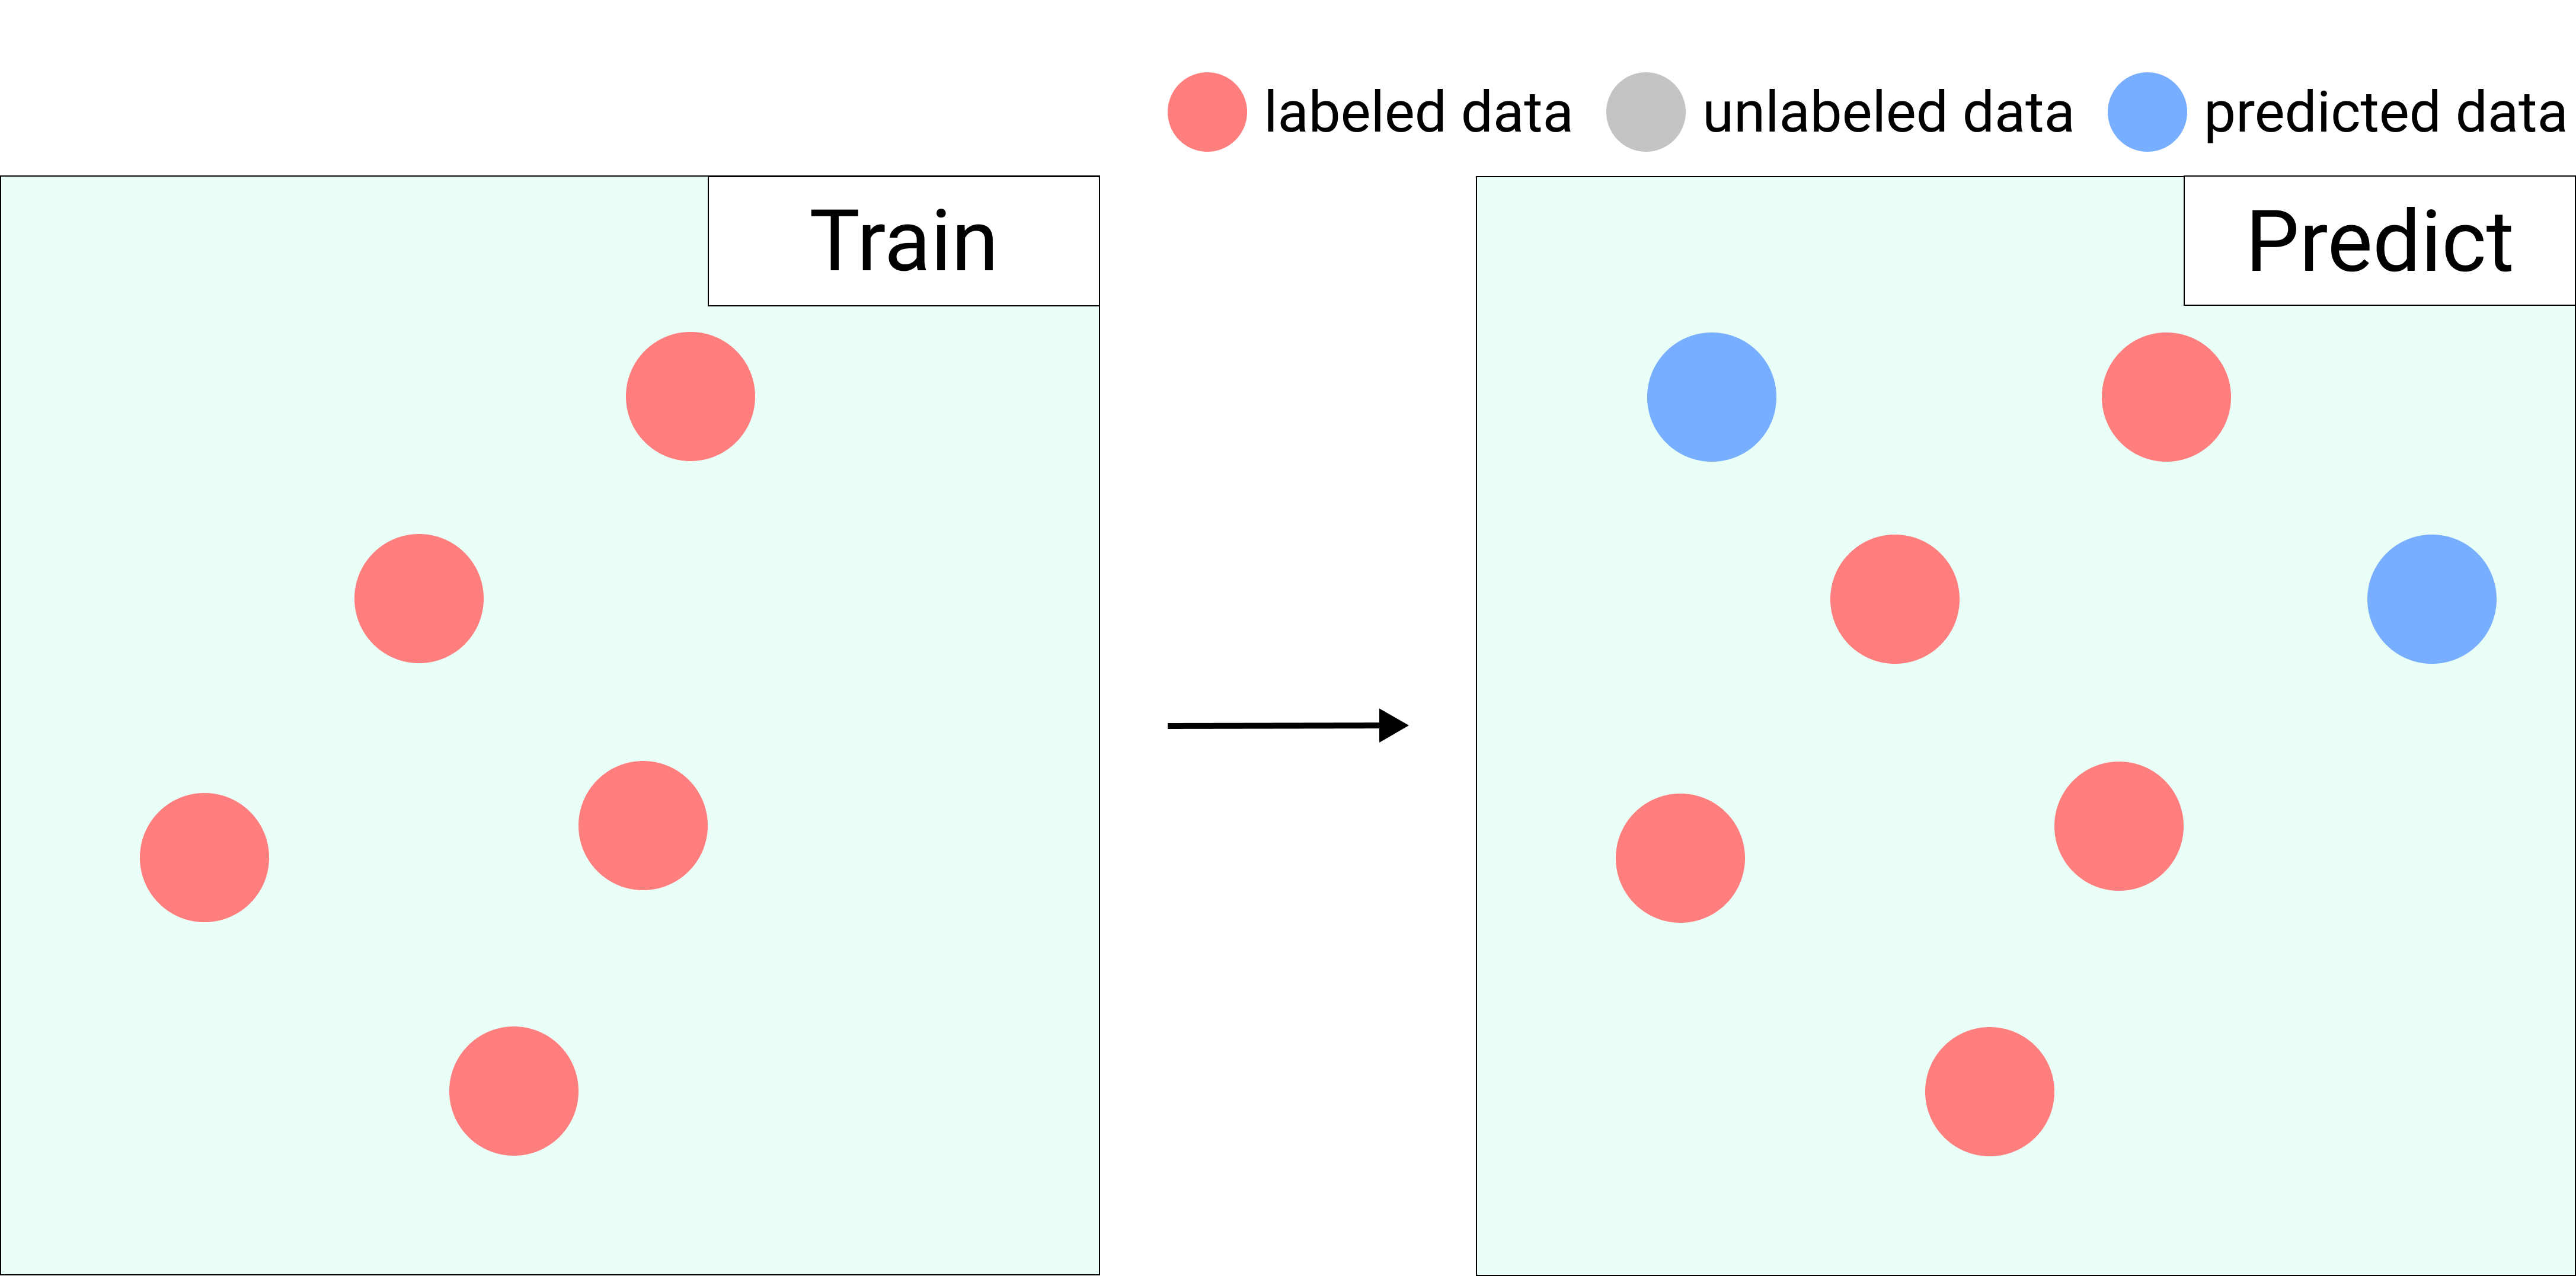
\includegraphics[width=\linewidth]
  {img/Inductive.jpg}
  \caption{帰納学習}
  \label{fig:Inductive}
\end{figure}


\subsection{fastText}
fastText\cite{bojanowski2017enriching}は Facebook AI Research によって開発された自然言語処理モデルである.このモデルを使用することで,単語埋め込みの生成やテキストの分類ができる.
本項では, Word2Vec で用いられている Skip-gram モデルについて説明し, その後, fastText で提案されたサブワードモデルについて説明する.
\subsubsection*{Skip-gram モデル}
Skip-gram モデルでは, サイズ W の単語の語彙が与えられ,単語はそのインデックス $w \in \{ 1,...,W \}$によって識別される場合, 各単語$w$のベクトル表現を学習することが目標となる.
分布仮説(周囲の単語によって単語の意味が形成されるという仮説)に基づき, 単語のベクトル表現はその文脈に現れる単語を予測して学習される.Skip-gram モデルでは式\ref{eq:fastLog}の対数尤度が最大になるように学習される.
\begin{equation}
  \label{eq:fastLog}
  \sum_{t=1}^{T} \sum_{c \in C_{t}} \log p(w_{c} | w_{t})
\end{equation}
ここで, T は与えられた文脈の長さ, $C_{t}$は注目単語$w_{t}$の周辺単語のインデックスの集合である.
注目単語と周辺単語のペアを実数にスコア付けする関数として$s(w_{t}, w_{c}) = \mathbf{u}_{w_{t}}^\mathsf{T}\mathbf{v}_{w_{c}}$(ここで,$\mathbf{u}_{w_{t}}, \mathbf{v}_{w_{c}}$は$w_{t}, w_{c}$に対応する単語ベクトル)が与えられるとする.
周辺単語が出現する確率$p(w_{c} | w_{t})$ の 1 つの選択肢として, 式\ref{eq:fastSoftmax}で示すソフトマックス関数が挙げられる.
\begin{equation}
  \label{eq:fastSoftmax}
  p(w_{c} | w_{t}) = \dfrac{e^{s(w_{t}, w_{c})}}{\sum_{j=1}^{W} e^{s(w_{t}, j)}}
\end{equation}
\par しかし, ソフトマックス関数を用いると計算量が大きくなる($W$は$10^5 〜 10^7$程度)という問題が存在する.
そのため,周辺単語の予測を,独立した二値分類問題の集合として構成する(Negative Sampling).
注目単語$w_{t}$に対して周辺単語$w_{c}$を正の例とし, 周辺単語以外の語彙からランダムに抽出した例を負の例とみなす.
その後,ロジスティック損失を用いて、式\ref{eq:loglike}に示す対数尤度を得る.

\begin{equation}
  \label{eq:loglike}
  \log (1 + e^{-s(w_{t}, w_{c})}) + \sum_{n \in \mathcal{N}_{t,c}} \log (1 + e^{s(w_{t}, n)})
\end{equation}
ここで, $\mathcal{N}_{t,c}$ が語彙からランダムに抽出した負の例の集合である.
最終的に, ロジスティク損失$l : x \mapsto \log(1+e^{-x})$とすると, Skip-gram モデルの目的は式\ref{eq:skipfin}を最小にすることである.
\begin{equation}
  \label{eq:skipfin}
  \sum_{t=1}^{T} \Biggl\lbrack \sum_{c \in C_{t}} l(s(w_{t}, w_{c})) + \sum_{n \in \mathcal{N}_{t,c}} l(-s(w_{t}, n))\Biggr\rbrack
\end{equation}

\par Skip-gram モデルでは各単語に個別のベクトル表現を用いており, 単語の内部構造は考慮していない.

\subsubsection*{サブワードモデル}
サブワードモデルでは, Skip-gram モデルで考慮されていなかった単語の内部構造を考慮するために, スコア付け関数を変更した.このモデルでは, 各単語の先頭と末尾に$<$と$>$を追加した,文字単位での$n$-gram を用いる. 例えば, \textsl{where}という単語に対して, $n=3$の場合の$n$-gram の集合は以下のようになる.
\centerline{$\{<$\textsl{wh, whe, her, ere, re}$>\}$}
このような, 文字単位での$n$-gram を利用したスコア付け関数は式\ref{eq:fastScore}で表される.
\begin{equation}
  \label{eq:fastScore}
  s(w,c) = \sum_{g\in \mathcal{G}_{w}} \mathbf{z}_{g}^\mathsf{T}\mathbf{v}_{c}
\end{equation}
ここで, $\mathcal{G}_{w}$は単語$w$の$n$-gram(実際には$n=3,4,5,6$のすべての$n$-gram)と$w$自身(\textsl{where}の例では$<$\textsl{where}$>$)の集合であり, $\mathbf{z}_{g}$は$n$-gram $g$のベクトル表現である.
\par サブワードモデルでは,スコア付け関数を変えたことによって単語の内部構造を考慮できるようになり, 出現頻度が低い語彙に対して, 信頼性の高い単語のベクトル表現を学習することができるようになった.
また, 単語の内部構造を考慮することにより, 未知語に対しても単語のベクトル表現を推論できるようになった.


\section{グラフニューラルネットワーク}\label{rel:GNN}
本節では, グラフニューラルネットワーク (GNN) に関する歴史や関連研究について述べる.
\subsection{GNNの歴史}
1997 年に Sperduti ら\cite{sperduti1997supervised}により, ニューラルネットワーク上で初めてグラフ構造が扱われた. この研究は初期の GNN の先駆的な研究となった.その後, Goriet ら\cite{gori2005anew},  Scarselli ら \cite{scarselli2009the} , Gallicchio ら \cite{gallicchio2010graph} により GNN に関する研究が行われてきた.
これらの研究は RNN のアーキテクチャを用いてグラフのノード埋め込みを学習することを目的としている(RecGNNs).
RecGNNs でのノードの更新は以下の 2 つの過程を繰り返す.
\begin{enumerate}
  \item 隣接ノード(+ノード自身)の状態を集約・解析 (メッセージパッシング)
  \item ノード自身の状態を更新
\end{enumerate}
周辺ノードの状態の集約はすべての層で同じ関数(かつ同じ重み)を用いて再帰的に行い, すべてのノードの状態が平衡状態になるまでノードの更新を続ける.
\par RecGNNs での第$l$層におけるノード$v$の出力$\mathbf{h}_{v}^{l}$は式\ref{eq:GNN}で表される.
\begin{equation}
  \label{eq:GNN}
  \mathbf{h}_{v}^{l}=\mathrm{Rec}(\mathbf{h}^{l-1}, \sum_{u \in \mathcal{N}(v)} W \mathbf{h}_{u}^{l})
\end{equation}
ここで, $\mathrm{Rec}$は RNN, LSTM などの再帰型ネットワーク, $\mathcal{N}(v)$はノード$v$の隣接ノードの集合である.
RecGNNs には計算コストが非常に高いという問題がある.
RecGNNs のメッセージパッシングの概念は, GCN に受け継がれている.
\subsection{Graph Convolutional Network}
Graph Convolutional Network (GCN) \cite{kipf2017semi} は,CNN のような畳み込み演算を GNN に適用したモデルである.1 層の GCN を用いるとそれぞれのノードが隣接するノードの情報を畳み込むという特徴がある. GCN は RecGNNs とは異なり, 層ごとに異なる重みを用いる.
隣接行列 $A$ と特徴行列 $X$ を GCN に与える入力とすると,GCN の第$l$層における出力$\mathbf{h}^{l}$は式\ref{eq:GCN}で表される.
\begin{equation}
  \label{eq:GCN}
  \mathbf{h}^{l}=f(\tilde{D}^{-\frac{1}{2}}\tilde{A}\tilde{D}^{-\frac{1}{2}}\mathbf{h}^{l-1}W_{1}^{(l-1)})
\end{equation}
ここで,$\tilde{A} = A + I_{N}$はノード自身へのエッジを追加した無向グラフの隣接行列であり,$I_N$は単位行列である.
$\tilde{D}_{ii} = \sum_{j} \tilde{A}_{ij}$であり,$W_{1}^{(l)}$は層に応じた学習可能な重み行列,$f(\cdot)$は$ReLU(\cdot) = \max (0, \cdot)$のような活性化関数である.
また,$H^{(0)}=X$となる.\par
GCN は層の数を増やしすぎると,全てのノードの埋め込みが同じ値に収束してしまい,性能が低下することがわかっている.

\subsection{GraphSAGE}
GraphSAGE は GCN を拡張したものであり, 帰納学習を行うことができるモデルである. GCN との違いとして, GraphSAGE では近傍ノードを抽出し, それを集約するための aggregate 関数を学習を学習する.GraphSAGE での前方伝播では, まずノードの近傍ノードを抽出し, サブグラフを作成する.
その後, 近傍ごとに異なる aggregate 関数を用いて, サブグラフ内のノードから特徴量を集約する.
最終的に集約した特徴量を元にラベルの推論を行う.前方伝播の過程を図\ref{fig:SAGE}に示す.

\begin{figure}
  \centering
  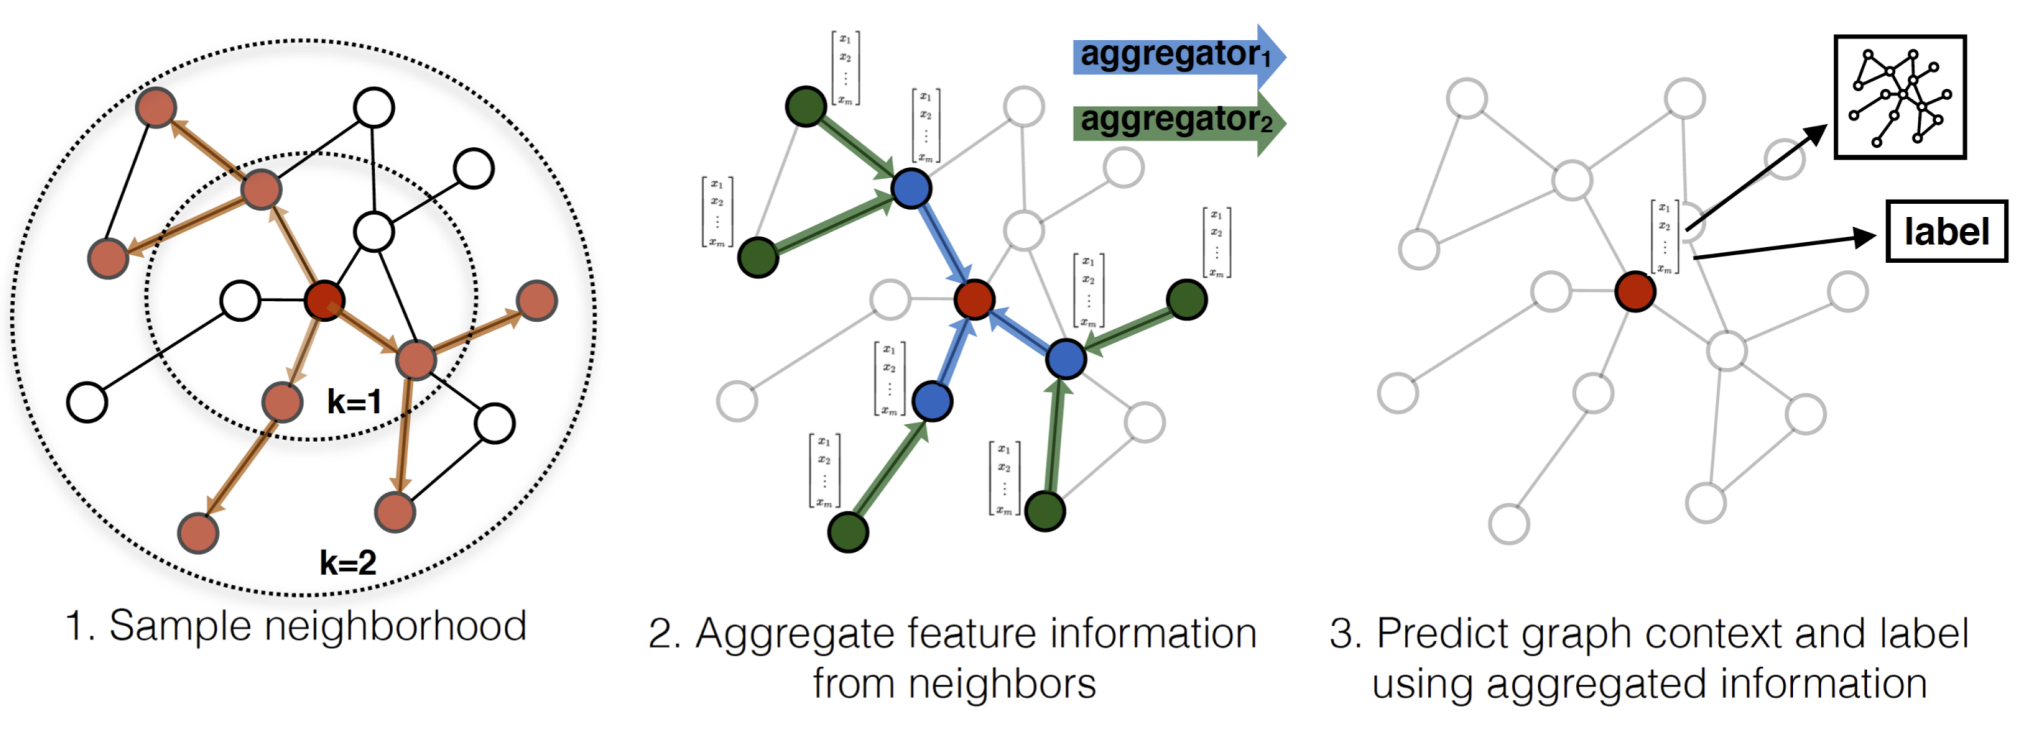
\includegraphics[width=\linewidth]
  {img/GraphSAGE.png}
  \caption{GraphSAGEの前方伝播 (\cite{hamilton2017inductive}より引用)}
  \label{fig:SAGE}
\end{figure}

aggregate 関数のアーキテクチャには 3 種類が存在する.
\subsubsection{Mean aggregator}
Mean aggregator を用いた場合, ノード$v$に対する GraphSAGE の第$l$層の出力$\mathbf{h}_{v}^{l}$は式\ref{eq:MeanAgg}で表される.
\begin{equation}
  \label{eq:MeanAgg}
  \mathbf{h}_{v}^{l} \leftarrow \sigma(\mathbf{W_{2}} \cdot \mathrm{MEAN} (\{ \mathbf{h}_{v}^{l-1}\} \cup \{ \mathbf{h}_{u}^{l-1} , \forall u \in \mathcal{N}(v) \}))
\end{equation}
ここで, $\mathbf{h}_{v}^{l}$は第$l$層でのノード$v$の埋め込みであり, $\mathbf{W_{2}}$は学習可能な重み行列, $\mathcal{N}(v)$はノード$v$の近傍ノード郡である.
このアーキテクチャは GCN と同様の処理を 帰納学習に対応させたものである.

\subsubsection{LSTM aggregator}
LSTM aggregator は, LSTM アーキテクチャに基づくより複雑な aggregator である. Mean aggregator に比べて, LSTM aggregator は表現力に優れている. しかし, LSTM は入力を逐次的に処理するため, ノードの入力順に応じて結果が変化する. そのため, ノードの近傍を不規則に並び替えることで, 非順序集合で LSTM を動作させた.

\subsubsection{Pooling aggregator}
Pooling aggregator は, 近傍ノードを全結合層に与え, その結果の中で最大となるものを選択する.これは, 式\ref{eq:PoolAgg}で表される.
\begin{equation}
  \label{eq:PoolAgg}
  \mathrm{AGGREGATE}_{k}^{\mathrm{pool}} = \max(\{ \sigma ( \mathbf{W_{2}}_{pool} \mathbf{h}_{u_{i}}^{k} + \mathbf{b} ), \forall u_{i} \in \mathcal{N}(v) \})
\end{equation}
ここで, $\sigma$ は非線形の活性化関数であり, $\mathbf{b}$はバイアスである.

\subsection{SimGNN}
SimGNN\cite{bai2019simgnn}は GNN を用いて近似的に Graph Edit Distance(GED)を求めるモデルである.グラフの入力ノードにはラベルが割り振られており,ノードの特徴量はラベルの One-Hot ベクトルとなる.
この手法では,入力グラフを複数層の GCN に与えることでノードレベルの埋め込みを生成した後,以下に示すアテンションモジュールを元にグラフレベルの埋め込みを生成する.
それらの非線形の変換をし, global graph context $c \in \mathbb{R}^{D}$を得る.
\begin{equation}c = \tanh (\frac{1}{N}W_{3}{\displaystyle \sum_{n=1}^{N}} u_{n})\end{equation}
ここで,$u_{n} \in \mathbb{R}^{D}$は入力ノード$n$の埋め込み,$D$はノードの埋め込みの次元,$W_{3} \in \mathbb{R}^{D \times D}$は学習可能な重み行列である.
$c$は重み行列を学習することで,グラフの全体的な構造及び特徴量を表すことができ,これに基づいて各ノードの重要度を計算することが可能となる.\par
ノード$n$に対しての重要度$a_{n}$の計算は,ノード$n$の埋め込み$u_{n}$と$c$の内積を計算した後,シグモイド関数$\sigma(x) = \frac{1}{1+exp(-x)}$を用いることで,重要度$a_{n}$を$(0,1)$の範囲に収める.
ここではグラフサイズを埋め込みに反映するため,全体の重要度を正規化しない.
重要度を計算した後,グラフレベルの埋め込み$h \in \mathbb{R}^{D}$を重み付きのノードの埋め込みの総和$h = \sum_{n=1}^{N}a_{n}u_{n}$で計算する.
アテンションモジュールについてまとめると式\ref{eq:Att}になる.
\begin{equation}
  \label{eq:Att}
  h = \sum_{n=1}^{N}\sigma(u_{n}^\mathsf{T}c)u_{n}= \sum_{n=1}^{N}\sigma(u_{n}^\mathsf{T} \tanh (\frac{1}{N}W_{3}\sum_{m=1}^{N}u_{m}))u_{n}
\end{equation}
AttentionModule から 2 つのグラフの埋め込み$h_{i} \in \mathbb{R}^{D}, h_{j} \in \mathbb{R}^{D}$が与えられた後,
それらの関係をモデル化するために,式\ref{eq:NTN} で表されるニューラルテンソルネットワークを用いる.
\begin{equation}
  \label{eq:NTN}
  g(h_{i}, h_{j})=f(h_{i}^\mathsf{T}W_{4}^{[1:K]}h_{j} + V \begin{bmatrix} h_{i}\\h_{j} \end{bmatrix} + b)
\end{equation}

ここで,$W_{4}^{[1:K]} \in R^{D \times D \times K}$は重み行列,$\begin{bmatrix} $ $ \end{bmatrix}$は結合操作,$V \in \mathbb{R}^{K\times2D}$は重みベクトル.
$b \in \mathbb{R}^{K}$はバイアスベクトル,$f(\cdot)$は$ReLU(\cdot) = \max (0, \cdot)$のような活性化関数である.
$K$は K は各グラフ埋め込みペアに対してモデルが生成する類似度の数を制御するハイパーパラメータである.\par


\subsection{Self-Attention Graph Pooling (SAGPool)}
Self-Attention Graph Pooling (SAGPool) \cite{lee2019self} はグラフプーリング手法の 1 つである. SAGPool を用いることで Self-Attention に基づいたノードの削減を行うことができる. この手法では, ノードの重要度は式\ref{eq:SAScore}で示される.
\begin{equation}
  \label{eq:SAScore}
  Z = \sigma (\tilde{D}^{-\frac{1}{2}}\tilde{A}\tilde{D}^{-\frac{1}{2}}X\Theta_{att})
\end{equation}
ここで, $\tilde{A} = A + I_{N}$はノード自身へのエッジを追加した無向グラフの隣接行列であり,$I_N$は単位行列である.
$\tilde{D}_{ii} = \sum_{j} \tilde{A}_{ij}$であり$\Theta_{att}$は SAGPool 層のパラメータである.
GCN を用いることで, グラフの特徴と構造情報の両方に基づいた重要度を得ることができる.
ノードの重要度を元に, Gao ら\cite{gao2019proceedings} によるノード選択方法を行うことで, 上位$\lceil kN \rceil$個のノードを保持する.ここで,$k \in (0,1)$はプーリングの割合である. 式\ref{eq:topk}はノード選択法を表す.
\begin{equation}
  \label{eq:topk}
  \mathrm{idx} = \textrm{top-rank}(Z, \lceil kN \rceil ), Z_{mask} = Z_{\mathrm{idx}}
\end{equation}
ここで, $\textrm{top-rank}$ は上位$\lceil kN \rceil$個のノードを返し, $\cdot_{\mathrm{idx}}$は$\mathrm{idx}$が示すノードのみの重要度である.
最終的に, 式\ref{eq:SAGPool}に表すように, 上位$\lceil kN \rceil$個のノードのみのグラフを作成する.
\begin{equation}
  \label{eq:SAGPool}
  X' = X_{\mathrm{idx},:}, X_{out} = X' \odot Z_{mask}, A_{out} = A_{\mathrm{idx,idx}}
\end{equation}
ここで, $X_{\mathrm{idx},:}$は$\mathrm{idx}$が示すノードの特徴量行列であり, $\odot$ はアダマール積 (要素ごとの積) であり, $A_{\mathrm{idx,idx}}$は$\mathrm{idx}$が示すノードの隣接行列である.

% 本原稿用の条件マクロ
% これ以降は削除しちゃダメ
\expandafter\ifx\csname MasterFile\endcsname\relax
\def\MasterFile{本原稿です}

% 参考文献
%% 本原稿用の条件マクロ
%章ごとにコンパイルできるようにするための設定.
%このマクロが定義されていない場合,チャプター内は個別のTEXソースとして扱われる.
\expandafter\ifx\csname MasterFile\endcsname\relax
\documentclass[a4j,12pt]{thesis} % 修論・卒論など (ページが右端にでる)   
\usepackage{mysettings}
\usepackage{url}

\begin{document}

\setlength{\baselineskip}{1.95zw}
\setlength{\textheight}{30\baselineskip}
\backmatter

\fi
% これより上は削除しちゃダメ
% 本原稿用の条件マクロここまで

%参考文献

\bibliographystyle{junsrt}
\bibliography{thesisB}

\clearpage


% 本原稿用の条件マクロ
% これ以降は削除しちゃダメ
\expandafter\ifx\csname MasterFile\endcsname\relax
\def\MasterFile{本原稿です}
\end{document}
\fi
% 本原稿用の条件マクロここまで


\bibliographystyle{junsrt}
\bibliography{thesisB}

\end{document}
\fi
% 本原稿用の条件マクロここまで
